\lab{Lorenz Equations}{Lorenz Equations}
\label{lab:lorenz}

\objective{Investigate the behavior of a system that exhibits chaotic behavior.
Demonstrate methods for visualizing the evolution of a system.}

Chaos is everywhere.
It can crop up in unexpected places and in remarkably simple systems, and a great deal of work has been done to describe the behavior of chaotic systems.
One primary characteristic of chaos is that small changes in initial conditions result in large changes over time in the solution curves.

\section*{The Lorenz System}
One of the earlier examples of chaotic behavior was discovered by Edward Lorenz.
In 1963, while working to study atmospheric dynamics he derived the simple system of equations
\begin{align*}
\frac{\partial x}{\partial t} &= \sigma \left(y - x\right) \\
\frac{\partial y}{\partial t} &= \rho x - y - x z \\
\frac{\partial z}{\partial t} &= x y - \beta z
\end{align*}
where $\sigma$, $\rho$, and $\beta$ are all constants.
After deriving these equations, he plotted the solutions and observed some unexpected behavior.
For appropriately chosen values of $\sigma$, $\rho$, and $\beta$, the solutions did not tend toward any steady fixed points, nor did the system permit any stable cycles.
The solutions did not tend off toward infinity either.
With further work, he began the study of what was called a strange attractor.
This system, though relatively simple, exhibits chaotic behavior.

\begin{problem}
\label{prob:lorenz_basic}
Use Mayavi's \li{plot3d} function to plot the trajectories of several points in the Lorenz system.
Use $\sigma = 10$, $\beta = \frac{8}{3}$, and $\rho = 28$.
Choose random initial values between $-15$ and $15$.
The result should look something like Figure \ref{fig:lorenz_plot}.
\end{problem}

\begin{figure}
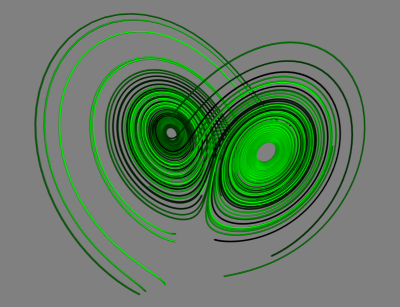
\includegraphics[width=\textwidth]{lorenz_plot.png}
\caption{Approximate solutions to the Lorenz equations for several random starting points.}
\label{fig:lorenz_plot}
\end{figure}

\section*{Animation in Mayavi}
Here we will take a brief diversion into some tools for plotting that will help us to visualize the evolution of systems like the one we are studying here.
Both Matplotlib and Mayavi allow for some kind of visualization.
% As of this writing, Mayavi's support for 3D plotting is much more robust than the plotting in Matplotlib, so we will encourage students to use it instead of Matplotlib.
Here we will work primarily with the animation functions in Mayavi, though similar functionality is available in Matplotlib.

\subsection*{Setting Data}
Said simply, most things you plot in Mayavi, allow you to change their data.
For things you plot using the basic built in plotting functions in the \li{mlab} api this can be done using the \li{set} and \li{reset} methods of the \li{mlab_source} attribute of the object created by the plotting function.
For example, the following short script will plot the curve $(t, \cos(t), 0)$, in spite of the fact that we originally plot the data corresponding to the curve $(t, \sin(t), 0)$.
\begin{lstlisting}
import numpy as np
from mayavi import mlab

x = np.linspace(- 2 * np.pi, 2 * np.pi)
y = np.sin(x)
z = np.zeros_like(x)
# Plot the first curve.
curve = mlab.plot3d(x, y, z)
# Change the y values.
curve.mlab_source.set(y=np.cos(x))
# Show the new curve.
mlab.show()
\end{lstlisting}

We can use this functionality in conjunction with some function decorators included in Mayavi to make a plot that continually evolves.
For example, we can continuously shift the phase of a curve like the one above using something like this:
\begin{lstlisting}
from mayavi import mlab
import numpy as np

def animate_sine(resolution=101, step=1, delay=20):
    # Compute the initial values for the curve.
    # Leave off the last point so we can update by rolling the entries of the array from
    # the end to the beginning.
    x = np.linspace(0, 4 * np.pi, resolution)[:-1]
    # Make the surface object and the initial plot.
    c = mlab.plot3d(x, np.sin(x), np.zeros_like(x), line_width=.2)
    # Use decorators to call the update the plot
    # periodically with a given time delay.
    # 'animate' is a generator that updates
    # the plot each time it is called.
    # The show decorator takes care of showing the figure.
    @mlab.show
    @mlab.animate(delay=delay)
    def animate():
        # Get 'y' back from the surface object.
        y = c.mlab_source.y
        # Update the plot at each iteration of this loop.
        while True:
            y = np.roll(y, step)
            c.mlab_source.set(y=y)
            yield
    # Run the animation on the figure.
    animate()
# Run the full animation.
animate_sine()
\end{lstlisting}

\begin{figure}
\begin{subfigure}{.49\textwidth}
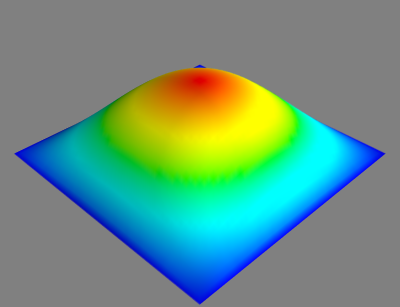
\includegraphics[width=\textwidth]{harmonic1.png}
\end{subfigure}
\begin{subfigure}{.49\textwidth}
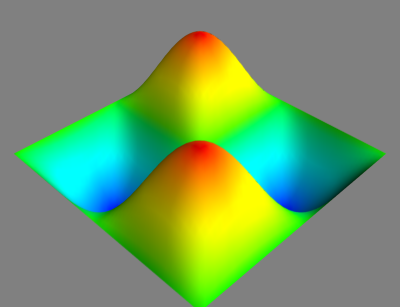
\includegraphics[width=\textwidth]{harmonic2.png}
\end{subfigure}
\caption{Simple surfaces we can animate with Mayavi.}
\label{fig:harmonic_animations}
\end{figure}

The \li{set} method can also be used on 3D surfaces.
The following two examples show how this is done.
The surfaces they animate are shown in Figure \ref{fig:harmonic_animations}.
\begin{lstlisting}
from mayavi import mlab
import numpy as np

def animate_harmonic(resolution=51, delay=25):
    # Make the initial data for the surface.
    x = np.linspace(0, np.pi, resolution)
    y = np.linspace(0, np.pi, resolution)
    x, y = np.meshgrid(x, y, copy=False)
    z = np.sin(x) * np.sin(y)
    # Plot the surface.
    # For now use zeros as the z values.
    # It will use the scalars values to select colors,
    # so we'll have it match the colors to the z values now.
    c = mlab.mesh(x, y, np.zeros_like(z), scalars=z)
    # Animate it by changing the 'z' values.
    @mlab.show
    @mlab.animate(delay=delay)
    def animate():
        # We'll have it oscillate between its current value
        # and the negative of its current value.
        # We'll have scale range from values of 0 to 2 * np.pi.
        scale = 0.
        while True:
            # Update the scale
            scale += .05
            # Cycle back toward 0 if necessary.
            if scale > 2 * np.pi:
                scale -= 2 * np.pi
            # Update the plot
            c.mlab_source.set(z = np.sin(scale) * z)
            yield
    # Run the animation on the figure.
    animate()
# Run the full animation.
animate_harmonic()
\end{lstlisting}

Here is an example that uses this same approach to plot a more generic oscillating surface.
\begin{lstlisting}
import numpy as np
from mayavi import mlab

def oscillate(x, y, z, delay=20):
    @mlab.show
    @mlab.animate(delay=delay)
    def animate(x, y, z):
        # Make the initial plot.
        surface = mlab.mesh(x, y, np.zeros_like(z), scalars=z)
        # Use this variable to scale it at each step in the animation.
        scale = 0.
        while True:
            scale += .05
            if scale > 2 * np.pi:
                scale -= 2 * np.pi
            # Update the 'z' values for the surface.
            surface.mlab_source.set(z = np.sin(scale) * z)
            yield
    # Run the animation
    animate(x, y, z)

# Here's another fun example.
# Construct the data for the plot.
x = np.linspace(0, np.pi)
y = np.linspace(0, np.pi)
x, y = np.meshgrid(x, y, copy=False)
z = np.sin(2 * x) * np.sin(2 * y)
# Run the animation.
oscillate(x, y, z)
\end{lstlisting}

\subsection*{Resetting Data}
The \li{set} method we have shown thus far is useful when we are changing the values of the data used in a plot, but it does not work when we need to change the \emph{shape} of the arrays involved as well.
Some times it is necessary to change the shapes of the arrays used for the plot.
To do this we must use the \li{reset} method.
Here is an example where we use the \li{reset} method to trace out a helix curve like the one shown in Figure \ref{fig:helix_animation}
\begin{lstlisting}
from mayavi import mlab
import numpy as np

def trace_helix(resolution=401, delay=10, step=1):
    z = np.linspace(0, 2, resolution)
    x = np.cos(4 * np.pi * z)
    y = np.sin(4 * np.pi * z)
    # Make a line to start from.
    # Note that the 'x', 'y', and 'z' coordinates for the curve must be contained in arrays or lists.
    # Only passing the coordinates of the first point will not work.
    # Notice how we are passing in the color.
    # The color is expected to be a tuple (not a list or array) representing RGB values for the desired color.
    c = mlab.plot3d(x[:1], y[:1], z[:1], line_width=.2, color=(1, 0, 0))
    # Set the camera position to a good angle for this plot.
    mlab.gcf().scene.camera.position = [3.95632052, 3.95626431, 4.95668558]
    mlab.gcf().scene.camera.focal_point = [2.27987766e-04, 1.71780586e-04, 1.00059305]
    mlab.gcf().scene.camera.clipping_range = [3.25443332, 11.39746923]
    @mlab.show
    @mlab.animate(delay=delay)
    def animate():
        scale = 0.
        for i in xrange(2 + step, z.size, step):
            # Reset the 'x', 'y', and 'z' coordinates for the graph.
            c.mlab_source.reset(x=x[:i], y=y[:i], z=z[:i])
            yield
    animate()
trace_helix()
\end{lstlisting}

\begin{figure}
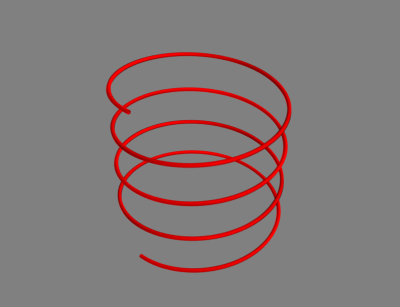
\includegraphics[width=\textwidth]{helix.png}
\caption{A simple curve we can animate using Mayavi.}
\label{fig:helix_animation}
\end{figure}

If you want to reset the zoom at each update so that the view updates to match the plot you can do the following
\begin{lstlisting}
from mayavi import mlab
import numpy as np

def trace_helix(resolution=401, delay=10, step=1):
    z = np.linspace(0, 2, resolution)
    x = np.cos(4 * np.pi * z)
    y = np.sin(4 * np.pi * z)
    c = mlab.plot3d(x[:1], y[:1], z[:1], line_width=.2, color=(1, 0, 0))
    @mlab.show
    @mlab.animate(delay=delay)
    def animate():
        scale = 0.
        for i in xrange(2 + step, z.size, step):
            c.mlab_source.reset(x=x[:i], y=y[:i], z=z[:i])
            # Reset the zoom at each iteration.
            mlab.gcf().scene.reset_zoom()
            yield
    animate()
trace_helix()
\end{lstlisting}

If you would like to find the proper configuration for the camera there are several different ways to do it.
One is to plot the full figure, and access the camera \li{scene}, \li{focal_point}, \li{clipping_range}, \li{viewing_angle}, and \li{view_up} attributes, save their values and use them to configure the plot as shown in the first example involving the helix.

You can also use the Mayavi pipeline window.
You can open this window by clicking the button at the top-right of the window where your plot appears.
If you click the red record button, move your plot to the position you want it to have, then stop the recording, you will be able to get the desired camera positioning.

\begin{problem}
\label{prob:lorenz_animation}
Write a Python function that animates the Lorenz system using Mayavi.
Have it accept a number of trajectories to plot, a final time value, a resolution for the plot, a stepping number (how many new points to include at each update of the plot), and a time delay to use between iterations.
Generate your starting points the same way you did in problem \ref{prob:lorenz_basic}.
Use different colors for each trajectory.
\end{problem}

We will now use animations to demonstrate that the Lorenz system is very sensitive to changes in the initial conditions.

\begin{problem}
\label{prob:lorenz_tol_sensitivity}
Write another Python function that produces a similar animation as the one in Problem \ref{prob:lorenz_animation}.
Use one initial guess, but solve the ODE system using the arguments \li{atol=1E-14} and \li{rtol=1E-12}, and then \li{atol=1E-15} and \li{rtol=1E-13} when you call \li{scipy.odeint}.
Have your function accept a final time value, a resolution for the curve, a stepping number, and a time delay to use between iterations.
What happens as you let your solution curves evolve over time?
Try running the simulation for longer periods of time.
% The solution curves should stay together for a while, then separate.
\end{problem}

\begin{problem}
Write another animation that plots a single solution set and another solution set with slightly perturbed initial conditions.
We will perturb the initial conditions by the smallest representable floating point value.
If \li{x0} is our first initial condition, let the second set of initial conditions, \li{x1}, be \li{x1 = y0 * (1. + 2.22E-16)}.
What happens as you let your solution curves evolve over time?
Try running the simulation for longer periods of time.
% The solution curves should stay together for a while, then separate.
\end{problem}

\section*{Lyapunov Exponents}
The Lyapunov exponent of a dynamical system is one measure of how chaotic a system is.
While there are more conditions for a system to be considered chaotic, one of the primary indicators of a chaotic system is \emph{extreme sensitivity to initial conditions}.
Strictly speaking, this is saying that a chaotic system is poorly conditioned.
Usually, in dynamical systems, the sensitivity to changes in initial conditions depends exponentially on the time the system is allowed to evolve.
If $\delta(t)$ represents the difference between two solution curves, when $\delta(t)$ is small, the following approximation holds.
\[\|\delta(t)\| \sim \|\delta(0)\| e^{\lambda t}\]
where $\lambda$ is a constant called the Lyapunov exponent.
For the Lorenz system, expirimentally it can be verified that $\lambda \approx .9$.

\begin{figure}
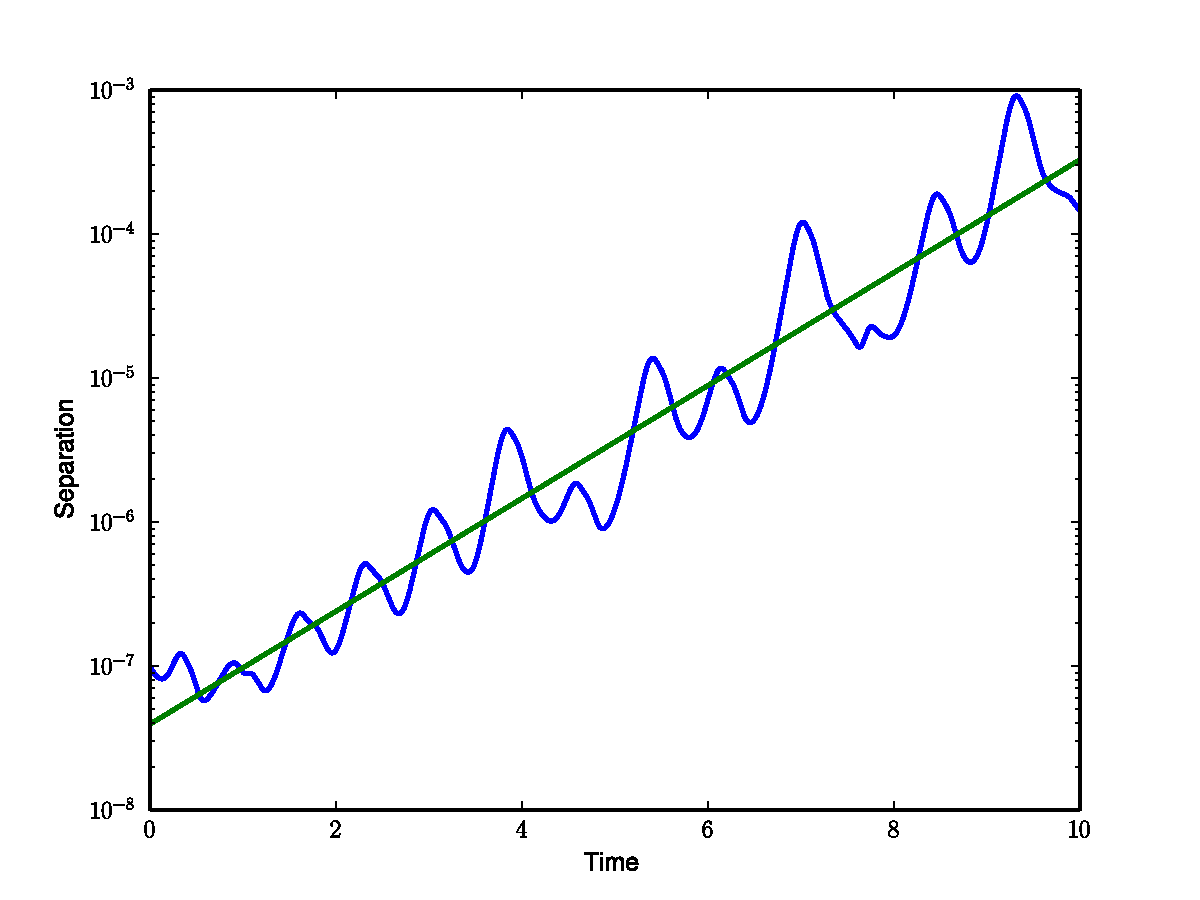
\includegraphics[width=\textwidth]{lyapunov_plot.pdf}
\caption{A semilog plot of the separation between two solutions to the Lorenz equations together with a fitted line that gives a rough estimate of the Lyapunov exponent of the system.}
\label{fig:lyapunov_exponent}
\end{figure}

\begin{problem}
Get a crude estimate of the lyapunov exponent for the Lorenz system.
Write a Python function that, finds an initial point on the strange attractor, runs the simulation to a given time $t$, and produces a semilog plot of the norm of the difference between the two solution curves.
Also have it plot an exponential line fitted to match the curve (this will be linear on the semilog plot).
Have it return a rough estimate of the Lyapunov exponent.
The output should be something like Figure \ref{fig:lyapunov_exponent}.

Note: In order to get a good estimate of the Lyapunov exponent, your initial guess should already lie on the strange attractor.
You can get a value on the attractor by running the system for a while to find a good initial guess.

Hint: To find the fitting line, take the logarithm of the norms of the differences, compute a linear fit, then take the exponential function of the resulting line.
The Lyapunov exponent will be approximately equal to the slope found by the linear regression.
\end{problem}